\PassOptionsToPackage{table}{xcolor}
\documentclass[12pt,letterpaper,twocolumn,openany,nodeprecatedcode,bg=none]{dndbook}
\usepackage[english]{babel}
\usepackage[utf8]{inputenc}
\usepackage{longtable,booktabs,array}
\usepackage{calc}
\usepackage{etoolbox}
\usepackage{caption}
\usepackage{float}
\usepackage{graphicx}
\usepackage{needspace}
\usepackage{tikz}

% Reset zebra striping at the start of every table
\AtBeginEnvironment{longtable}{\rowcolors{1}{white}{gray!10}\small}
\AtBeginEnvironment{table}{\rowcolors{1}{white}{gray!10}}

\providecommand{\pandocbounded}[1]{#1}
\providecommand{\tightlist}{%
  \setlength{\itemsep}{0pt}\setlength{\parskip}{0pt}}

\captionsetup{labelformat=empty}
\setcounter{secnumdepth}{0}
\setlength{\parindent}{0pt}
\setlength{\parskip}{0.5\baselineskip}
\setlength{\headheight}{15pt}

% Prevent orphaned subsections
\let\oldsubsection\subsection
\renewcommand{\subsection}[1]{%
  \needspace{5\baselineskip}%
  \oldsubsection{#1}%
}

\begin{document}
\onecolumn

      \title{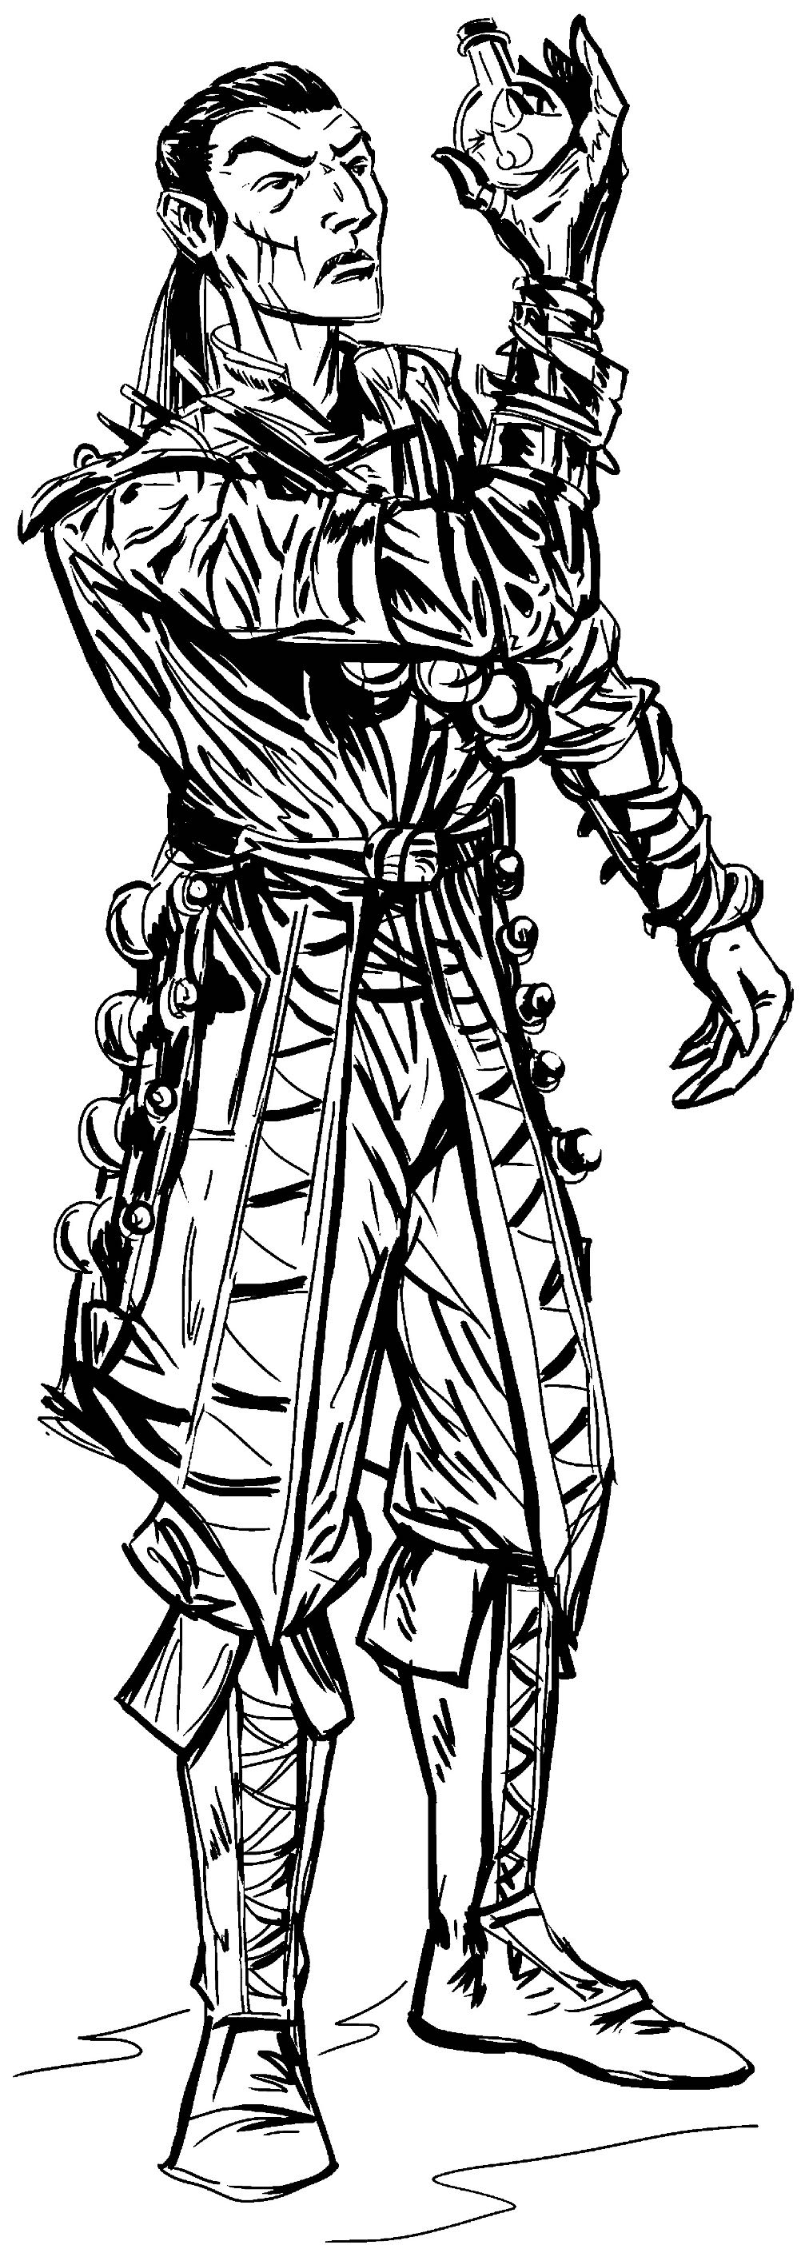
\includegraphics[width=0.9\textwidth,height=0.55\textheight,keepaspectratio]{alchemist.png}\\[1.5cm]Viper}
  \author{Class Handbook}
\date{}
\maketitle

\clearpage
\thispagestyle{empty}
\null\vfill
\begin{center}{\Large\itshape Your trusty class handbook for fantasy
gaming.}\end{center}
\vfill


\clearpage
\twocolumn

\section{Viper}\label{viper}

\subsection{Core Viper Traits}\label{core-viper-traits}

\needspace{11\baselineskip}

{\def\LTcaptype{none} % do not increment counter
\begin{table}[!htbp]
\centering
\begin{tabular}{@{}
  >{\raggedright\arraybackslash}p{(\linewidth - 2\tabcolsep) * \real{0.3467}}
  >{\raggedright\arraybackslash}p{(\linewidth - 2\tabcolsep) * \real{0.6533}}@{}}
\toprule\noalign{}
\begin{minipage}[b]{\linewidth}\raggedright
\textbf{Primary Ability}
\end{minipage} & \begin{minipage}[b]{\linewidth}\raggedright
Dexterity
\end{minipage} \\
\midrule\noalign{}
\textbf{Hit Points} & 1d4 \\
\textbf{Saving Throw Proficiencies} & Dexterity, Intelligence \\
\textbf{Skill Proficiencies} & Choose 4 skills \\
\textbf{Weapon Proficiencies} & Choose 3 categories \\
\textbf{Starting Equipment} & Padded Jacket, 2 Daggers, Sabre,
Poisoner's Kit \\
\bottomrule\noalign{}
\end{tabular}
\end{table}
}

\subsection{Viper Features}\label{viper-features}

\needspace{20\baselineskip}

{\def\LTcaptype{none} % do not increment counter
\begin{table}[!htbp]
\centering
\begin{tabular}{@{}
  >{\raggedright\arraybackslash}p{(\linewidth - 4\tabcolsep) * \real{0.1282}}
  >{\raggedright\arraybackslash}p{(\linewidth - 4\tabcolsep) * \real{0.2821}}
  >{\raggedright\arraybackslash}p{(\linewidth - 4\tabcolsep) * \real{0.5897}}@{}}
\toprule\noalign{}
\begin{minipage}[b]{\linewidth}\raggedright
Level
\end{minipage} & \begin{minipage}[b]{\linewidth}\raggedright
Proficiency
\end{minipage} & \begin{minipage}[b]{\linewidth}\raggedright
Class Features
\end{minipage} \\
\midrule\noalign{}
1 & +2 & Poisoner \\
2 & +2 & --- \\
3 & +2 & Ability Bonus, Ambusher \\
4 & +2 & --- \\
5 & +2 & --- \\
6 & +2 & --- \\
7 & +2 & Ability Bonus \\
8 & +2 & --- \\
9 & +3 & Deadly Venom \\
10 & +3 & --- \\
\bottomrule\noalign{}
\end{tabular}
\end{table}
}

\subsection{Level 1: Poisoner}\label{level-1-poisoner}

If you have a poisoner's kit, as an action you can mix a poison and
apply it to a weapon (or an arrow or similar ammunition) or a drink. The
drink remains poisoned for 10 minutes. The weapon remains poisoned for 2
rounds.

If the poison is ingested or the weapon hits a creature, the target must
make a Constitution save opposed by your Intelligence check. If the save
fails, the target takes damage based on your level.

\needspace{11\baselineskip}

{\def\LTcaptype{none} % do not increment counter
\begin{table}[!htbp]
\centering
\begin{tabular}{@{}
  >{\raggedright\arraybackslash}p{(\linewidth - 2\tabcolsep) * \real{0.3158}}
  >{\raggedright\arraybackslash}p{(\linewidth - 2\tabcolsep) * \real{0.6842}}@{}}
\toprule\noalign{}
\begin{minipage}[b]{\linewidth}\raggedright
Level
\end{minipage} & \begin{minipage}[b]{\linewidth}\raggedright
Poison Damage
\end{minipage} \\
\midrule\noalign{}
1--2 & 1d10 \\
3--4 & 2d10 \\
5--6 & 3d10 \\
7--8 & 4d10 \\
9--10 & 5d10 \\
\bottomrule\noalign{}
\end{tabular}
\end{table}
}

\subsection{Level 3: Ability Bonus}\label{level-3-ability-bonus}

You gain a +1 bonus to two different abilities of your choice.

\subsection{Level 3: Ambusher}\label{level-3-ambusher}

You have advantage on initiative rolls. If you surprise your enemies,
you can take an extra action on your turn.

\subsection{Level 7: Ability Bonus}\label{level-7-ability-bonus}

You gain a +1 bonus to two different abilities of your choice.

\subsection{Level 9: Deadly Venom}\label{level-9-deadly-venom}

Your poisons are incredibly deadly. You can spend 1 minute to apply a
poison rather than an action. If you do so, the poison gains one of the
following benefits:

\begin{itemize}
\tightlist
\item
  Double its damage dice.
\item
  If the target fails its saving throw, it is paralyzed. Repeat the
  saving throw at the end of each of its turns, ending the paralysis if
  it succeeds.
\end{itemize}

\onecolumn

\clearpage
\thispagestyle{empty}
\begin{center}
\vspace*{\fill}
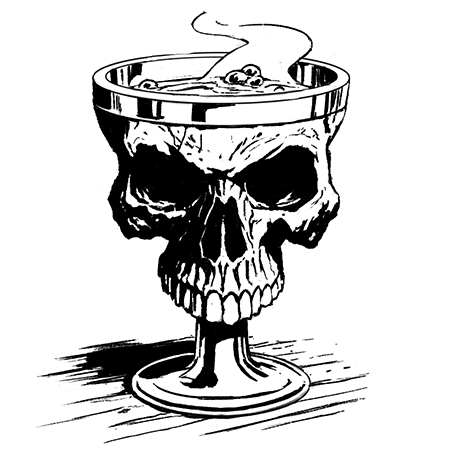
\includegraphics[width=0.7\textwidth,keepaspectratio]{skullPoison.jpg}\par
\vspace{0.4cm}
{\itshape Drink up, looks perfectly harmless\ldots{}}\par
\vspace*{\fill}
\end{center}

\end{document}